\documentclass[a4paper, 10pt]{article}
%\usepackage{fontspec}
%\setmainfont{Lato}
\usepackage{pgf}
\usepackage{eurosym}
\usepackage{graphicx}
\usepackage{wasysym}
\usepackage{hyperref}
\usepackage{listings}
\usepackage{pxfonts}
\usepackage{verbatim}
\usepackage{color}
\usepackage{xcolor}
\usepackage{wrapfig}
\usepackage{enumitem}
\usepackage{booktabs}
\usepackage{gensymb}
\usepackage{tabularx}
\usepackage{currfile}

\hypersetup{
    bookmarks=true,         % show bookmarks bar?
    unicode=true,          % non-Latin characters in Acrobat’s bookmarks
    pdftoolbar=true,        % show Acrobat’s toolbar?
    pdfmenubar=true,        % show Acrobat’s menu?
    pdffitwindow=true,     % window fit to page when opened
    pdftitle={Assessments},    % title
    pdfauthor={Paul Vesey},     % author
    pdfsubject={Advanced Graphics Assignment },   % subject of the document
    pdfcreator={},   % creator of the document
    pdfproducer={xelatex}, % producer of the document
    pdfkeywords={'Graphics' }, % list of keywords
    pdfnewwindow=true,      % links in new PDF window
    colorlinks=true,       % false: boxed links; true: colored links
    linkcolor=violet,          % color of internal links (change box color with linkbordercolor)
    citecolor=magenta,        % color of links to bibliography
    filecolor=red,      % color of file links
    urlcolor=blue           % color of external links
}

\setlength\parindent{0pt}
\begin{document}

\lstset{language=HTML,
				basicstyle=\small,
				breaklines=true,
        numbers=left,
        numberstyle=\tiny,
        showstringspaces=false,
        aboveskip=-20pt,
        frame=leftline
        }
				
\begin{table}%
	\begin{minipage}{0.4\textwidth}%
			
\includegraphics[width=1\textwidth]{./img/LITlogo.jpg}
	\end{minipage}
	\qquad
	\centering
	\parbox{0.4\textwidth}{
		\begin{large}			
			\begin{tabular}{| r | l |} \hline
				Subject: & \textbf{Advanced Graphics}\\
								 & \textbf{\& Visualisation}\\
				Course: & \textbf{Interior Design Y3}\\
				Session: & \textbf{Autumn 2020}\\
				Lecturer: & \textbf{Paul Vesey \footnotesize{BEng, MIE, HDip}}\\
				Filename: & \footnotesize{\currfilename}\\
				\hline
			\end{tabular}
		\end{large}			
	}
\end{table}
\vspace{0.25cm}	

\begin{flushleft}
\Large\textbf{Assignment 2 - Hotel Room Renders using VRay (15\%)}\\
\end{flushleft}

This assignment is based on a simple hotel room design.  You have been provided with a 3DS Max model of the room which also includes 3 lights and 5 camera views.  You have also been provided with a pdf of the room design. \\
\\
In this assignment you are required to improve the interior design of the space and to create 5 photo-realistic renders using VRay. You may use materials and assets from sources of your own choosing; however you must include a text file in the `import' that contains details of where you sources the assets.\\
\\
Your key deliverables are 5 high quality renders of the interior space. Three or four images are to be of the main bedroom space, and one or two images are to be of the en-suite bathroom.\\
\\
To assist you in this assignment, I suggest the following work-flow:\\

\begin{enumerate}
	\item Examine the design drawings and decide on your improvements.
	\item Source 3DS files from TurboSquid, Polantis or similar as necessary.
	\item Import, scale and place your objects and run test renders.
	\item Create and modify materials as necessary.
	\item Run numerous test renders and add additional lights as necessary for the design and illumination of the space
	\item Create final renders.
\end{enumerate}



\begin{figure}[hb]
	\centering
		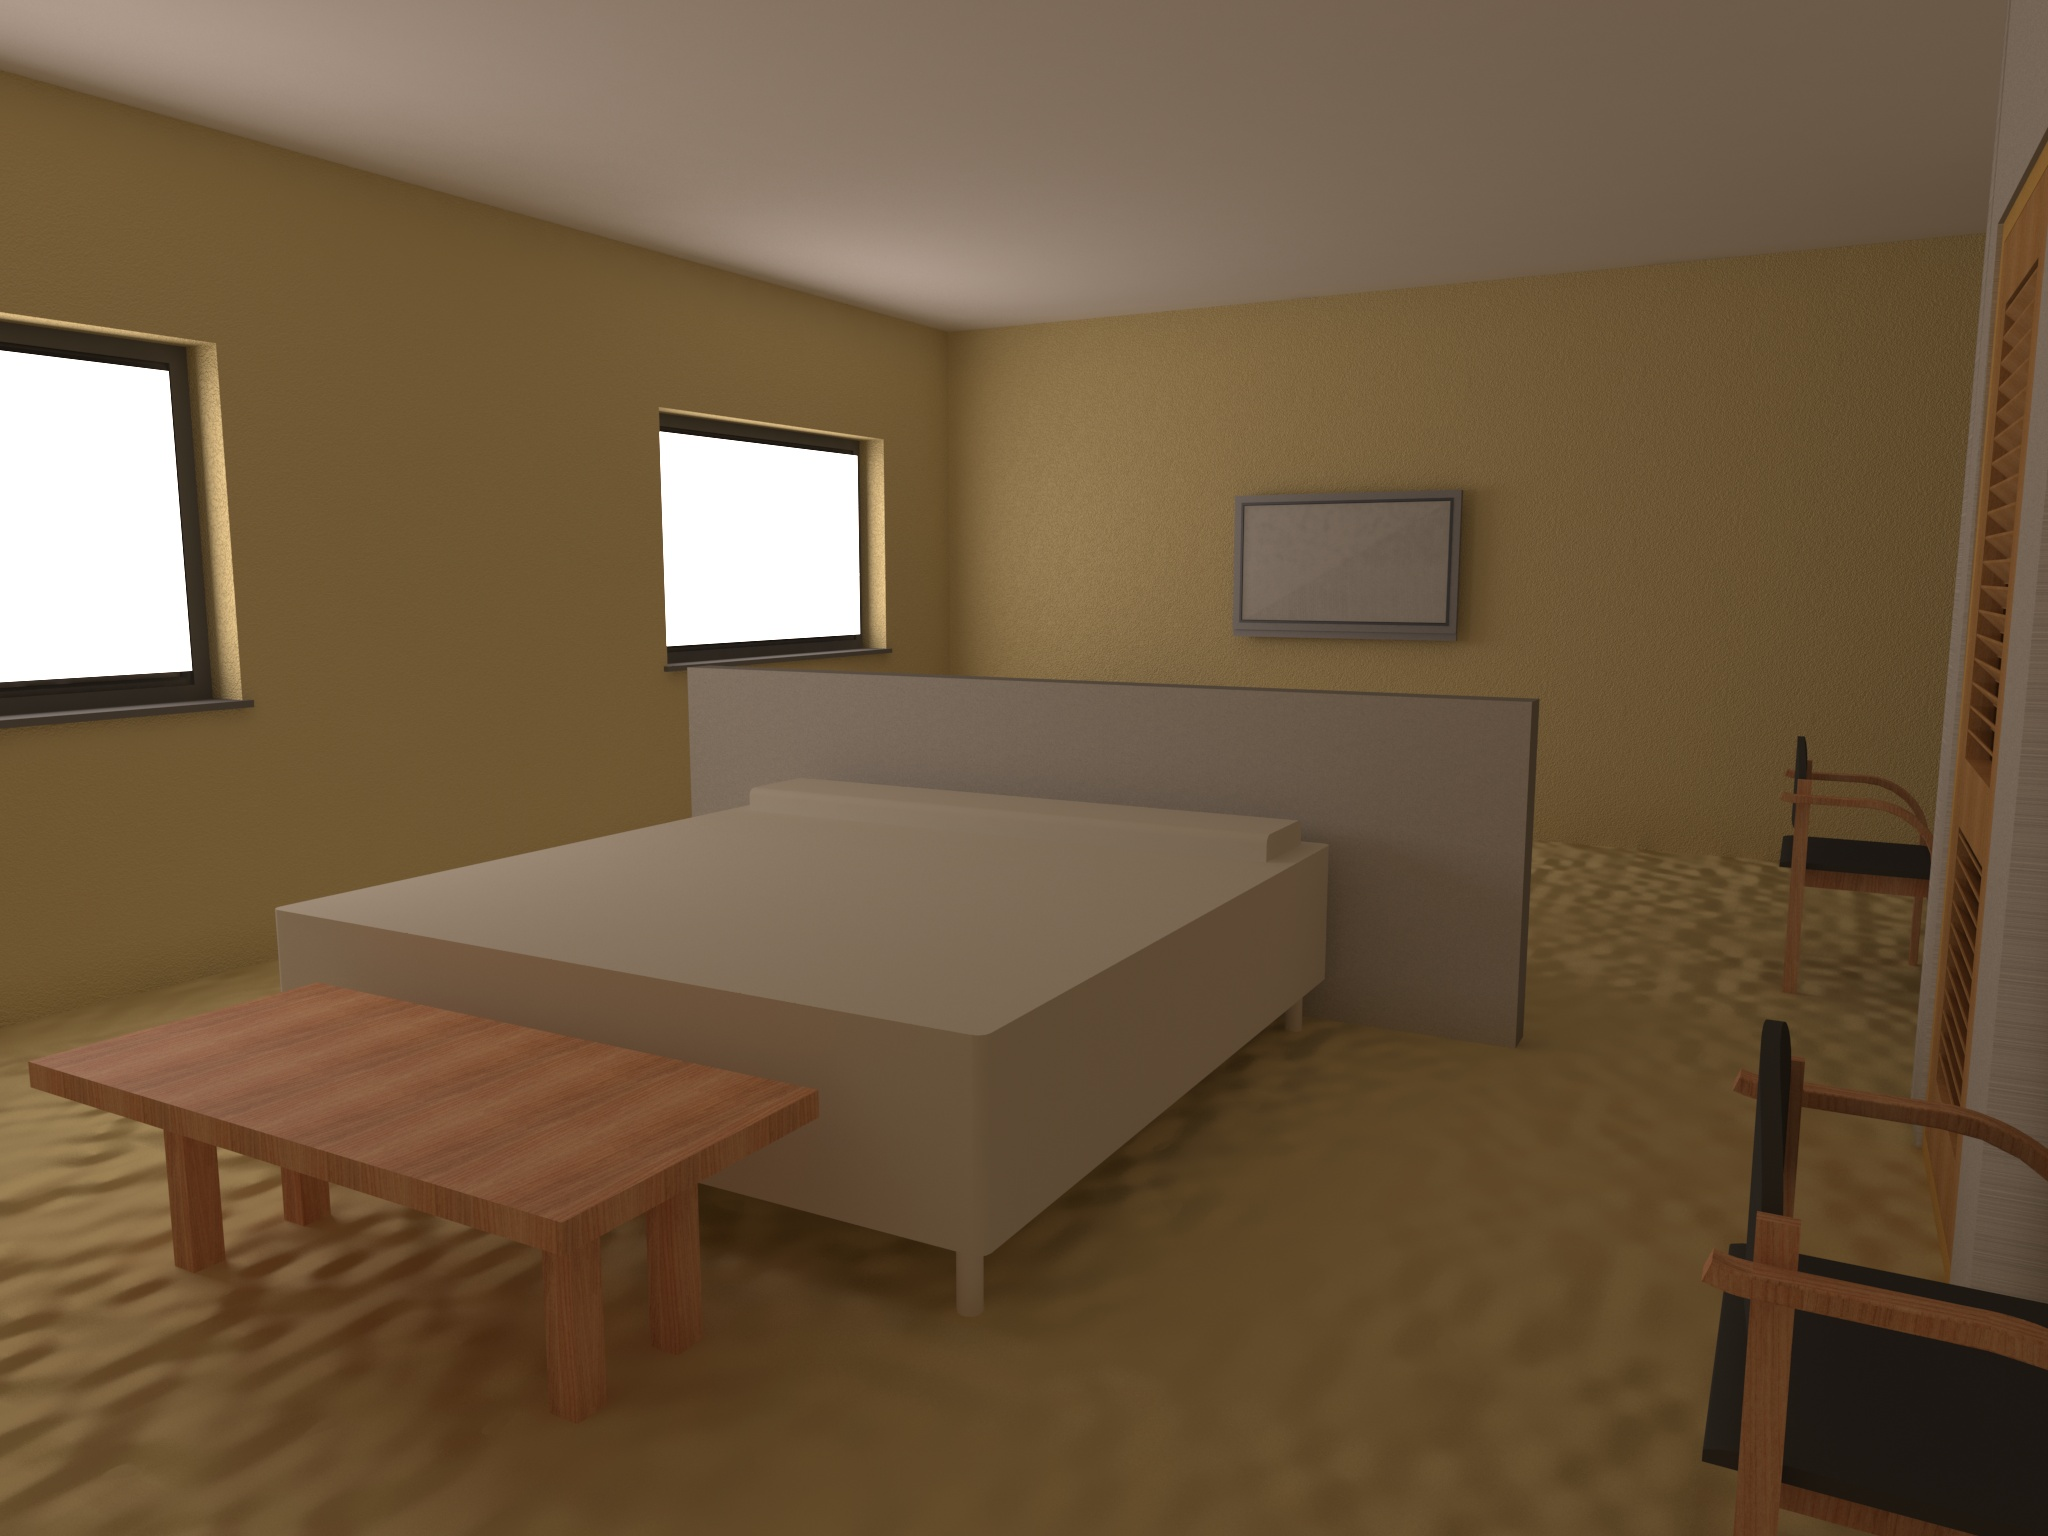
\includegraphics[width=10cm]{img/HotelRoomCamera1.jpg}
		\caption{Camera 1 Render}
	\label{fig:Cam1}
\end{figure}


\begin{figure}[hb]
	\centering
	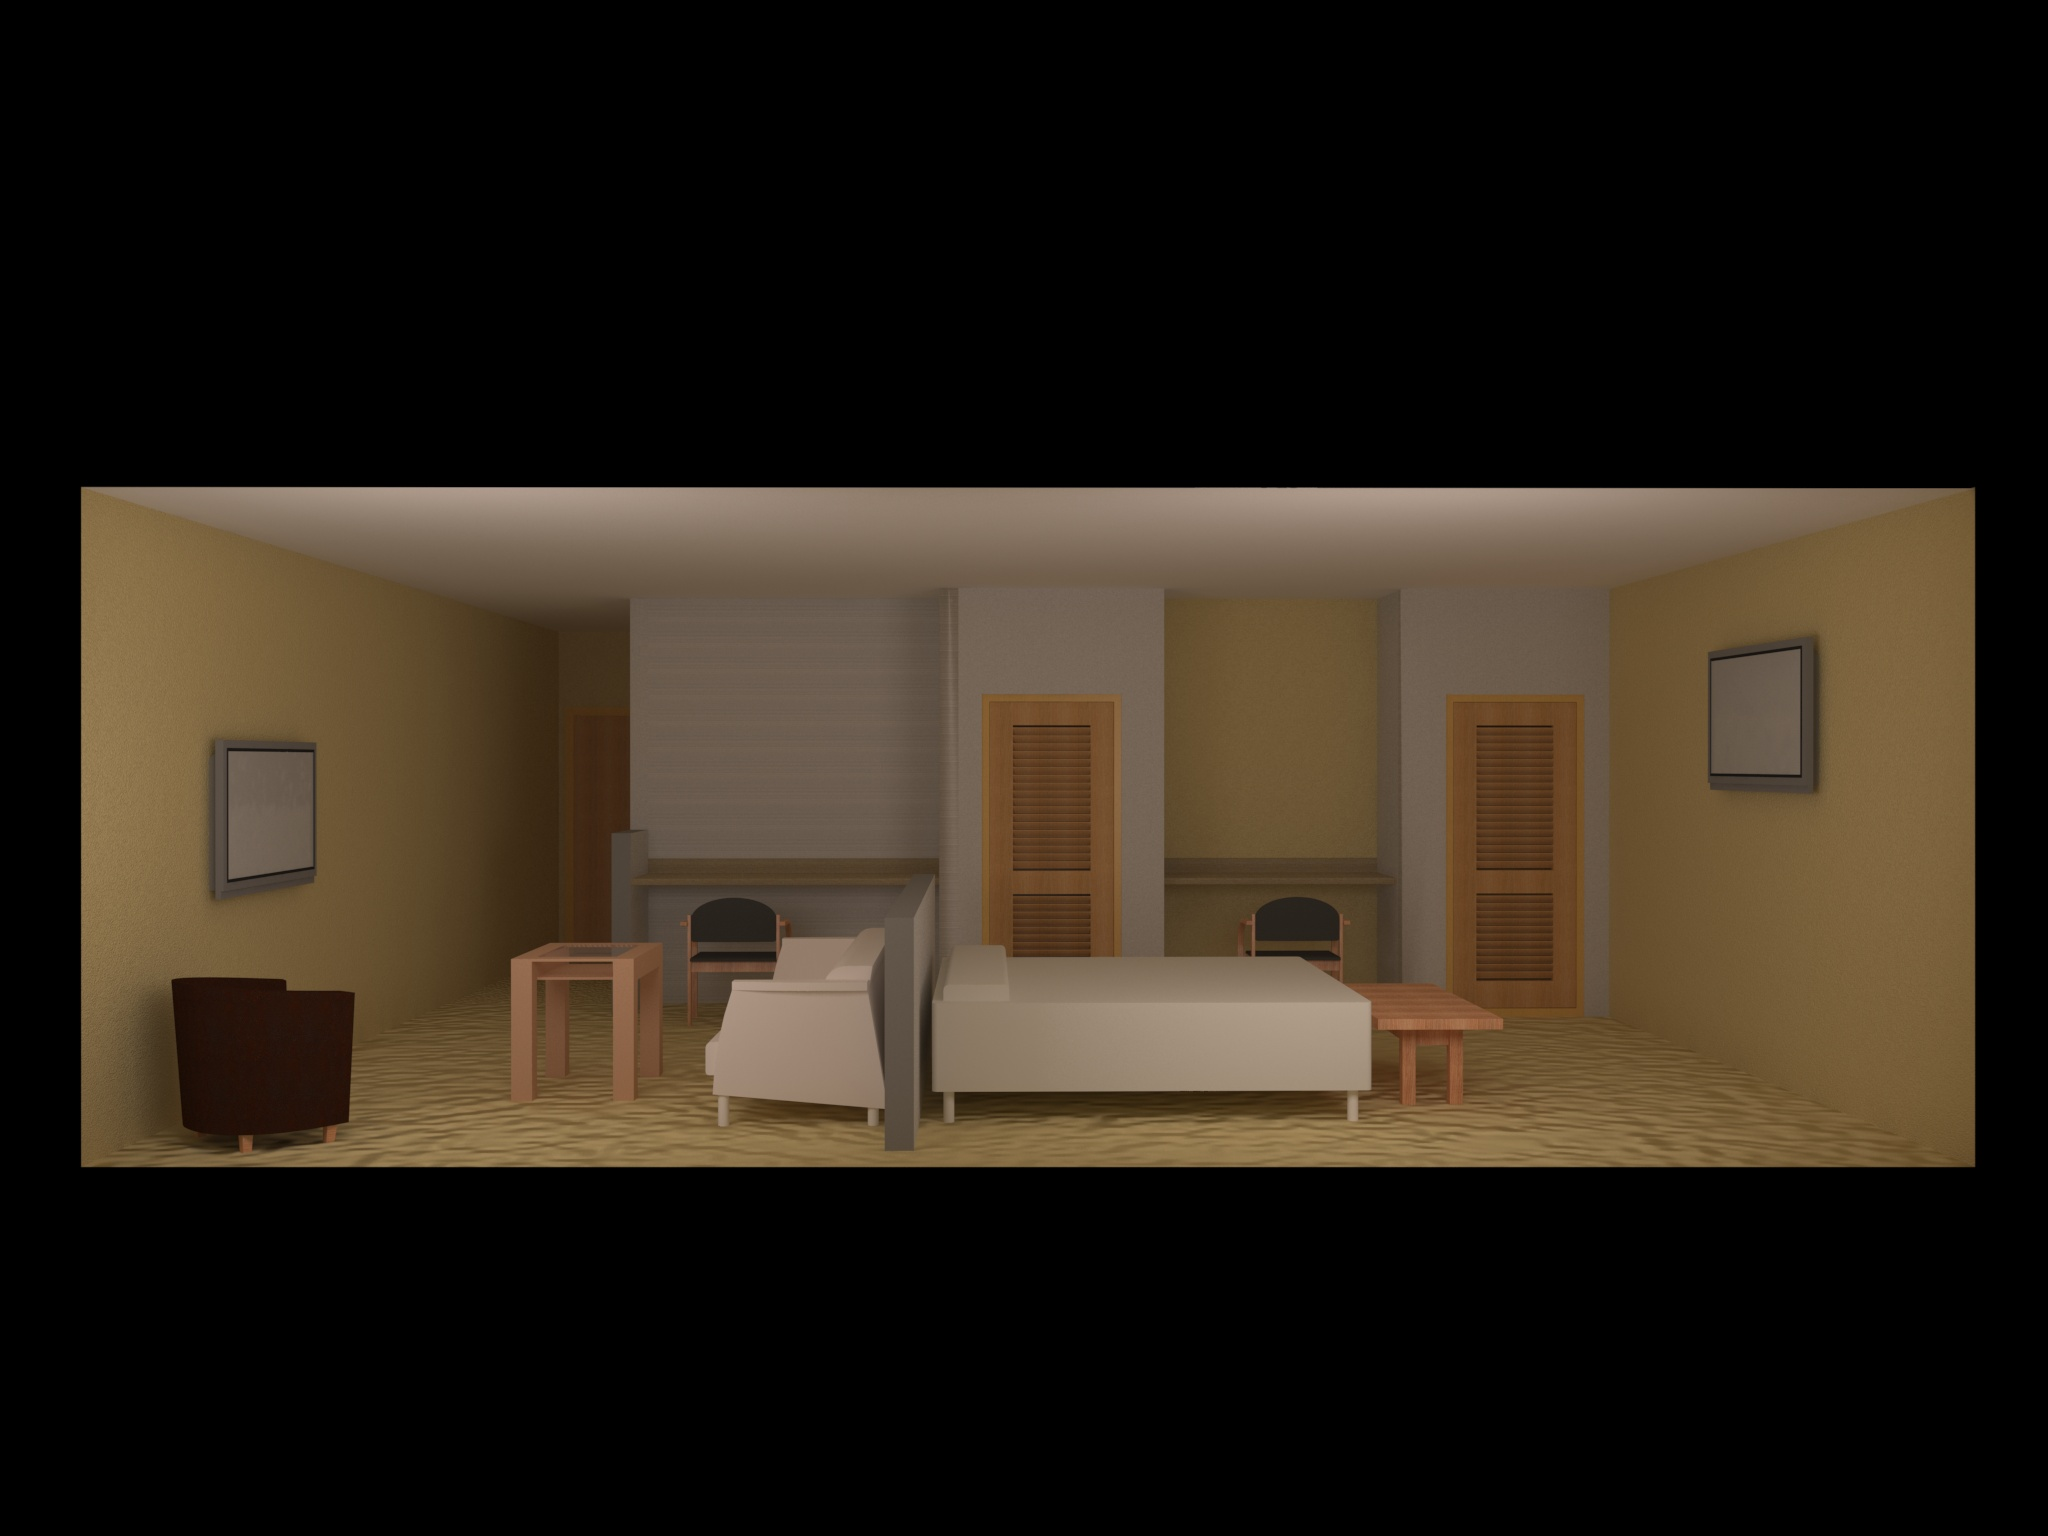
\includegraphics[width=10cm]{img/HotelRoomCamera2.jpg}
	\caption{Camera 2 Render}
	\label{fig:Cam2}
\end{figure}

\begin{figure}[hb]
	\centering
	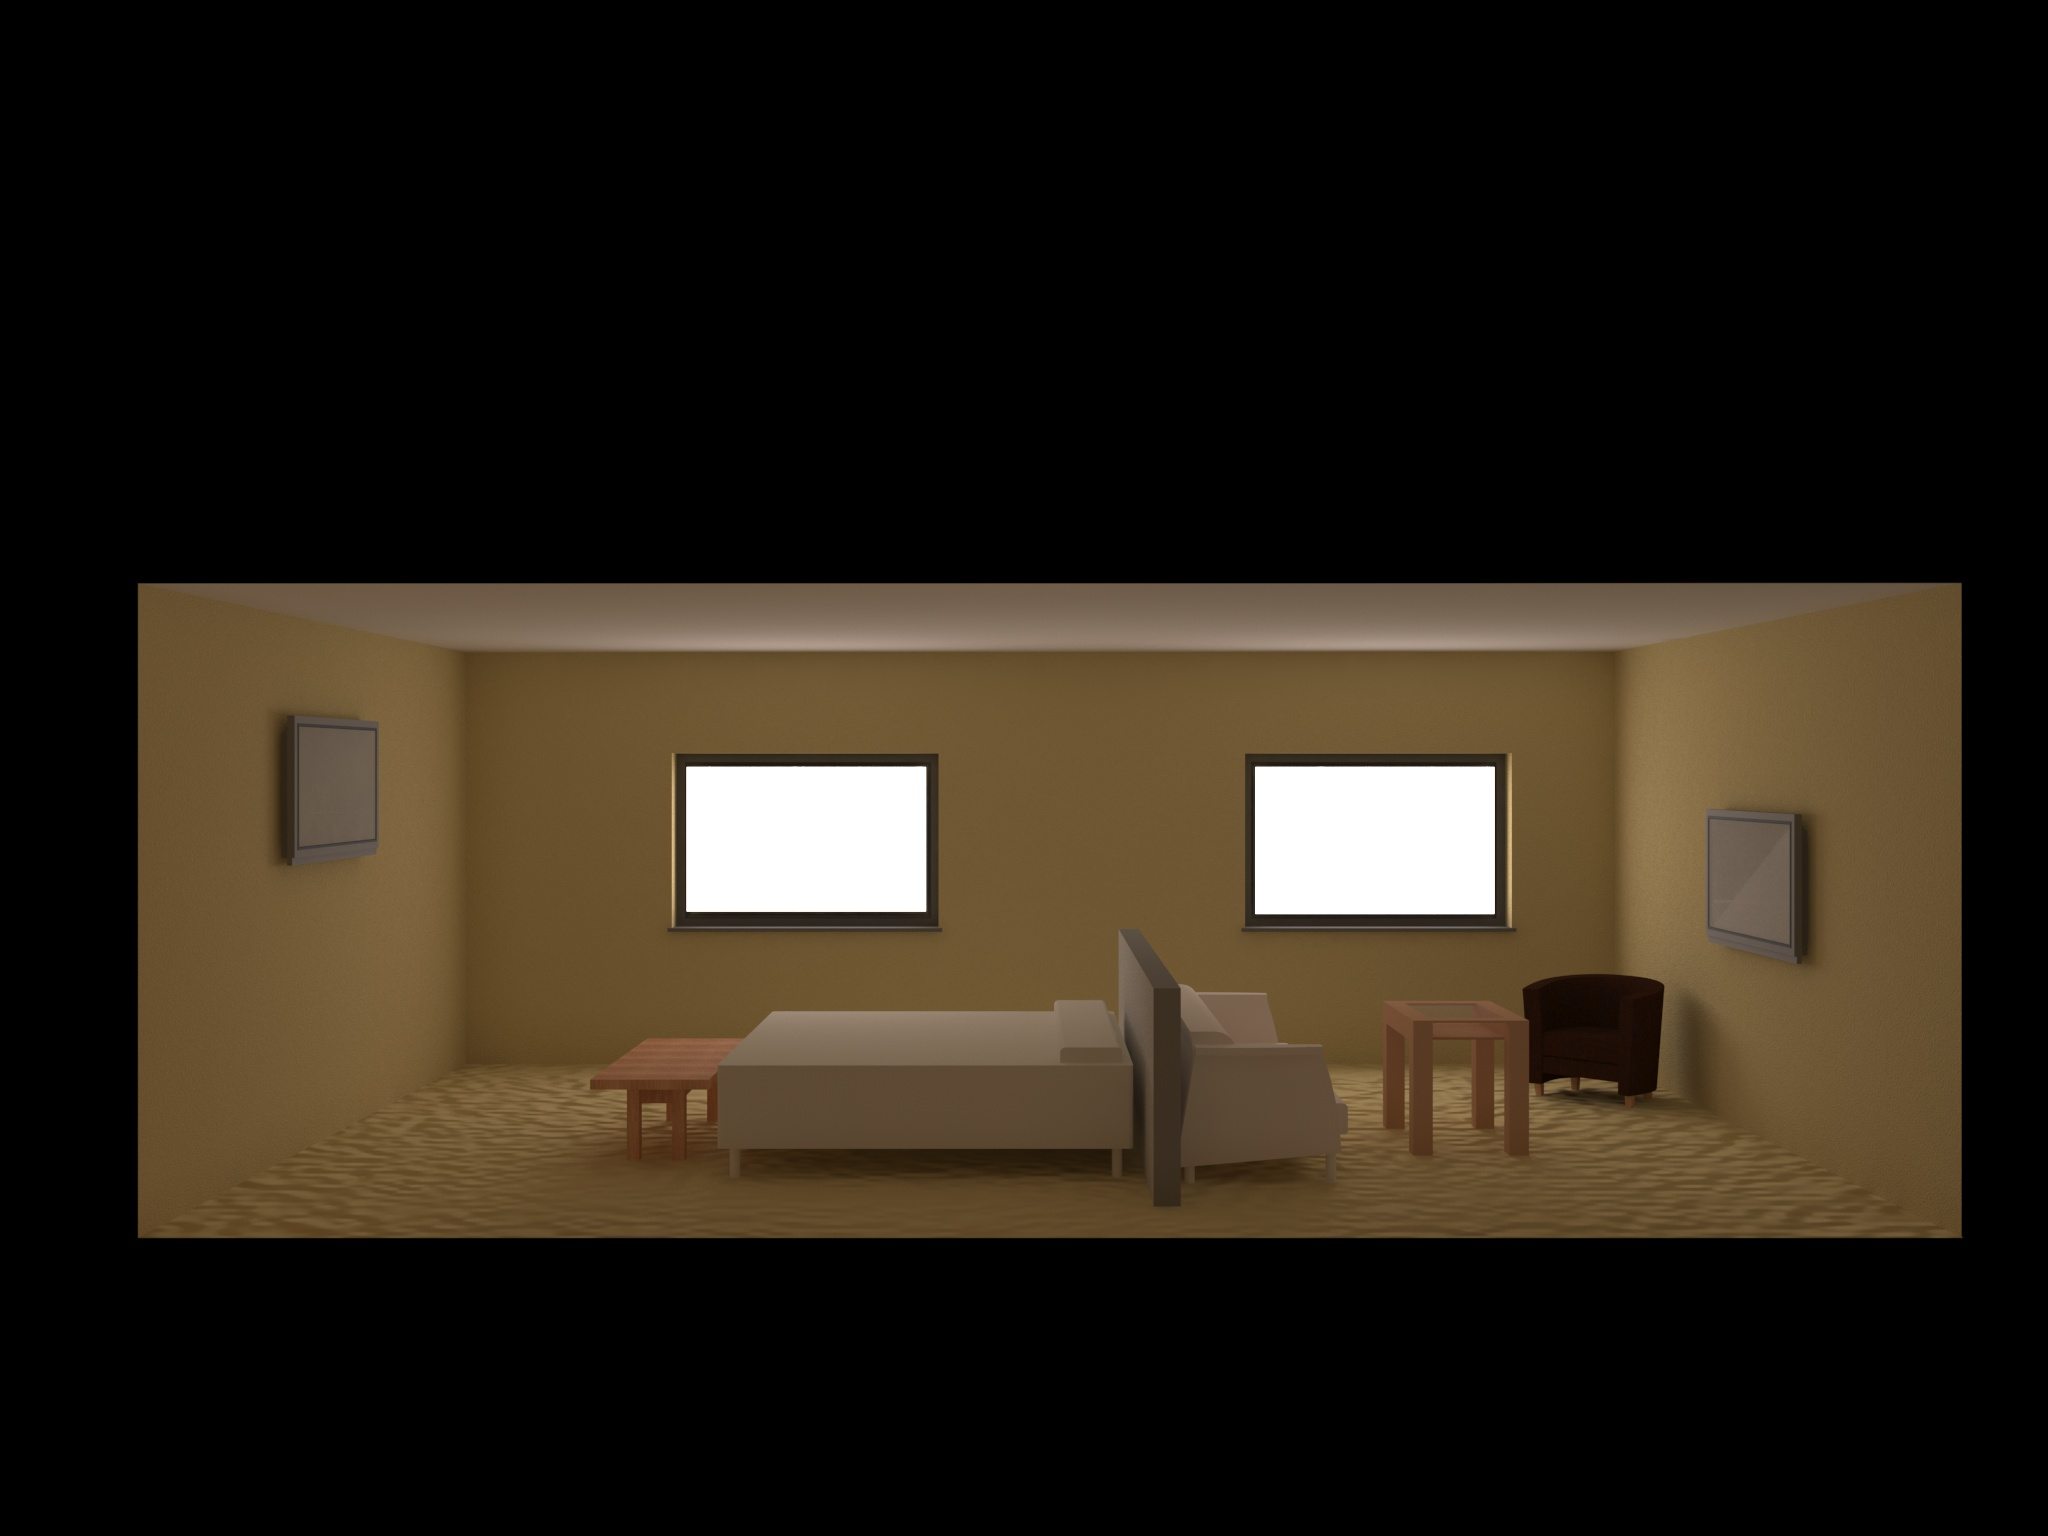
\includegraphics[width=10cm]{img/HotelRoomCamera3.jpg}
	\caption{Camera 3 Render}
	\label{fig:Cam3}
\end{figure}

\begin{figure}[hb]
	\centering
	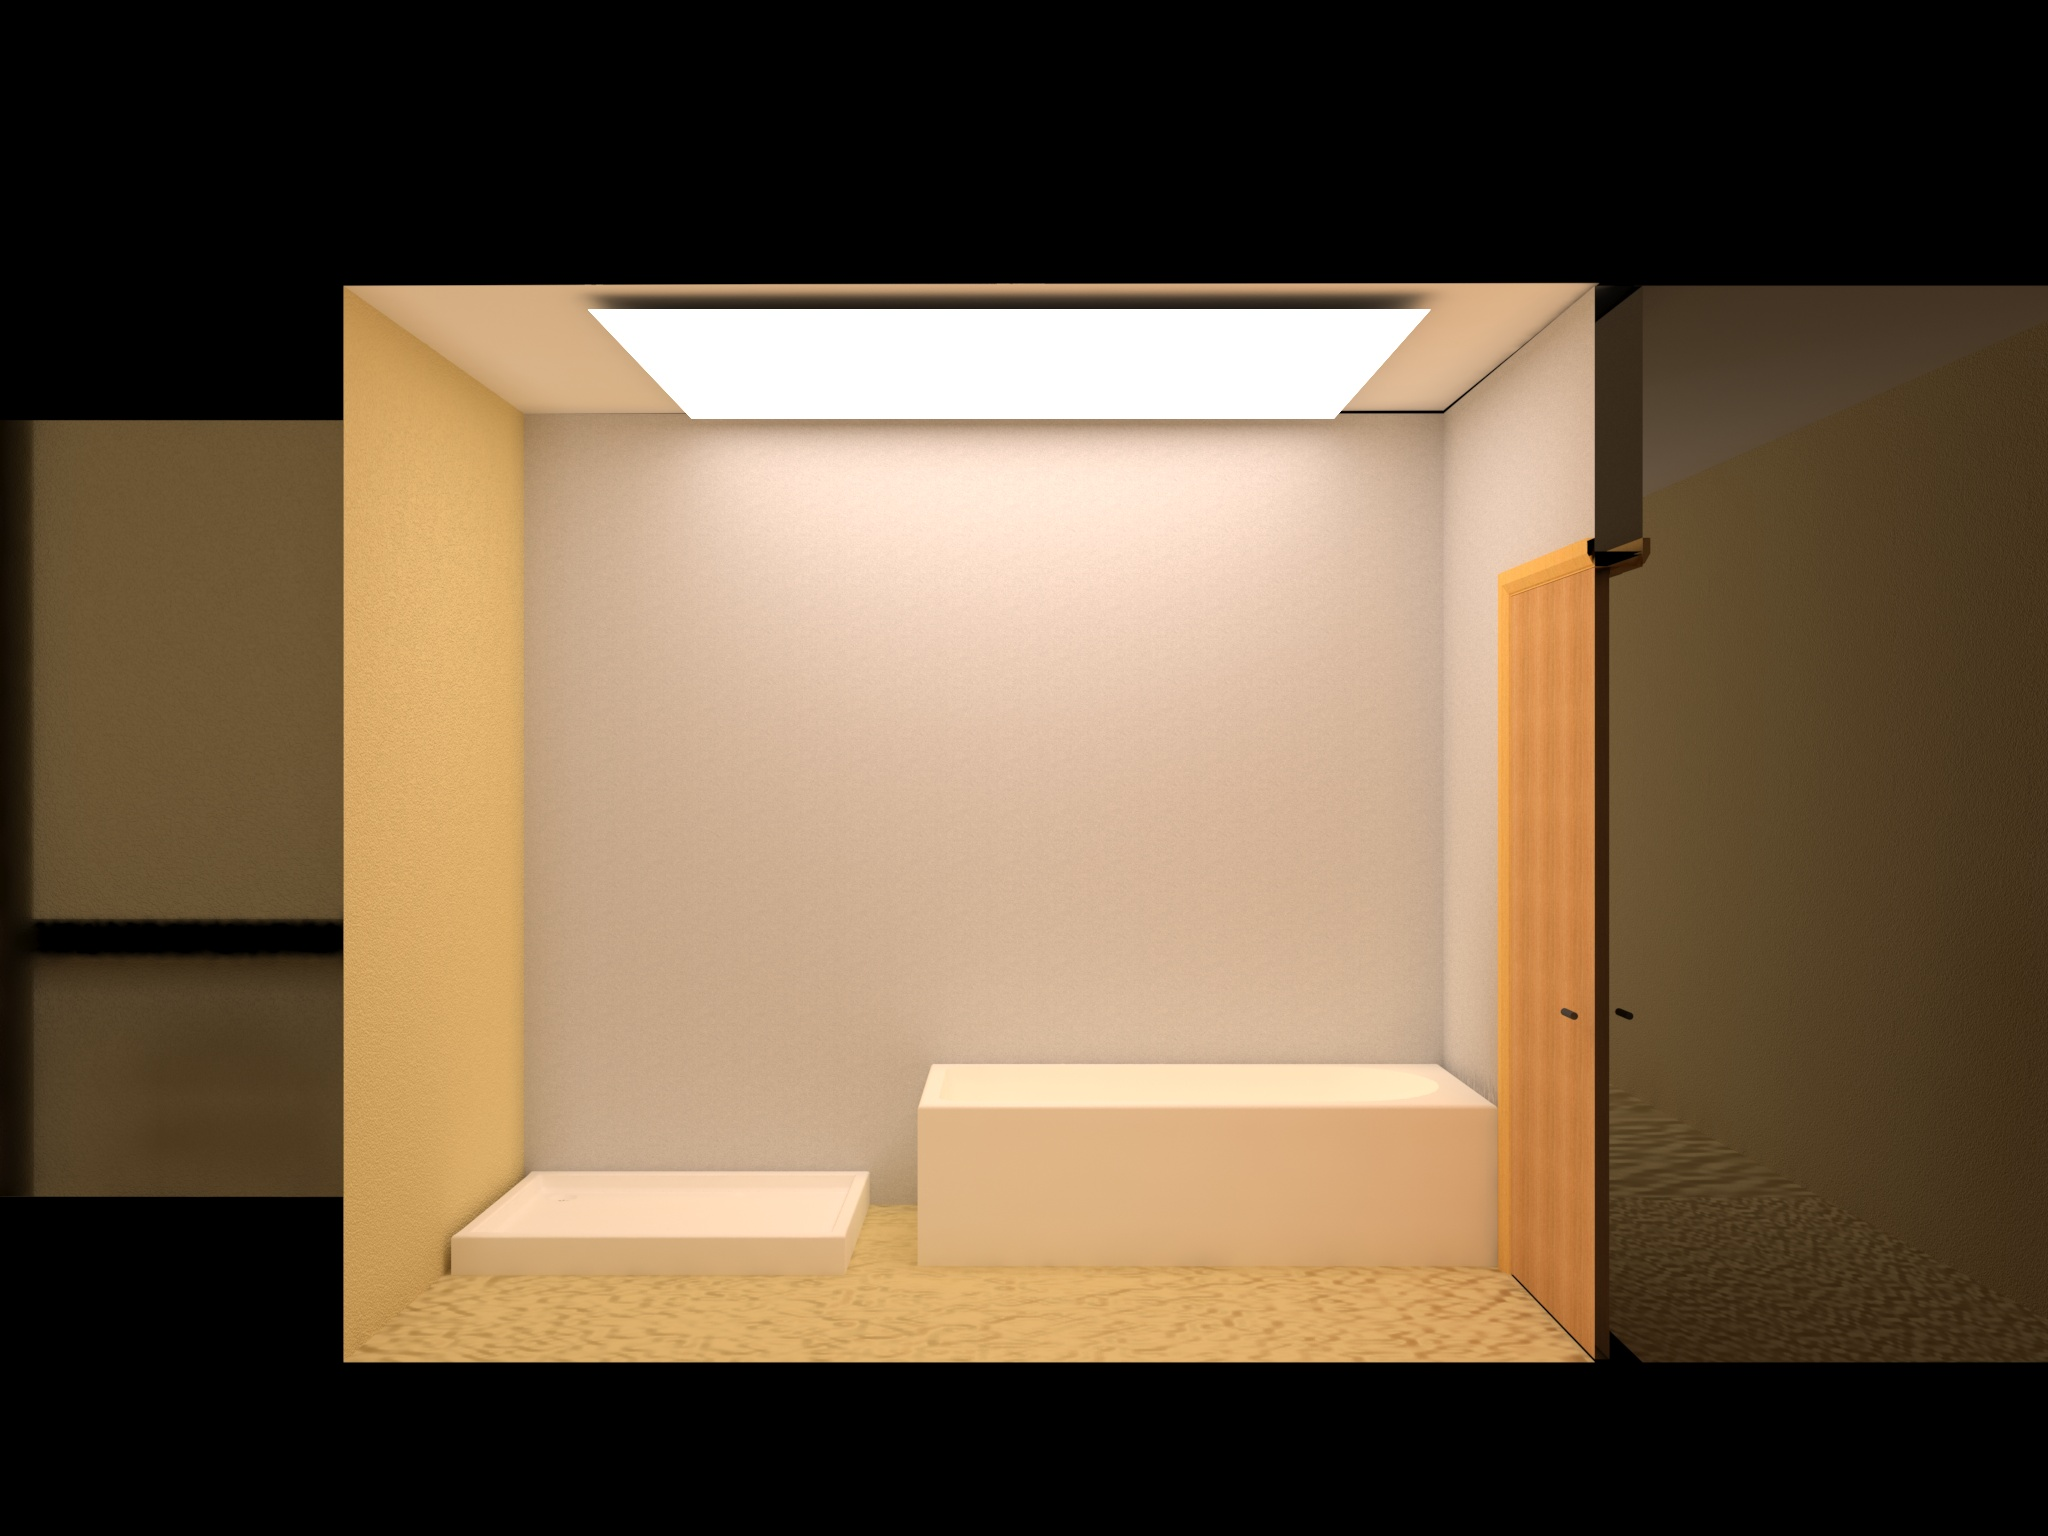
\includegraphics[width=10cm]{img/HotelRoomCamera4.jpg}
	\caption{Camera 4 Render}
	\label{fig:Cam4}
\end{figure}

\begin{figure}[hb]
	\centering
	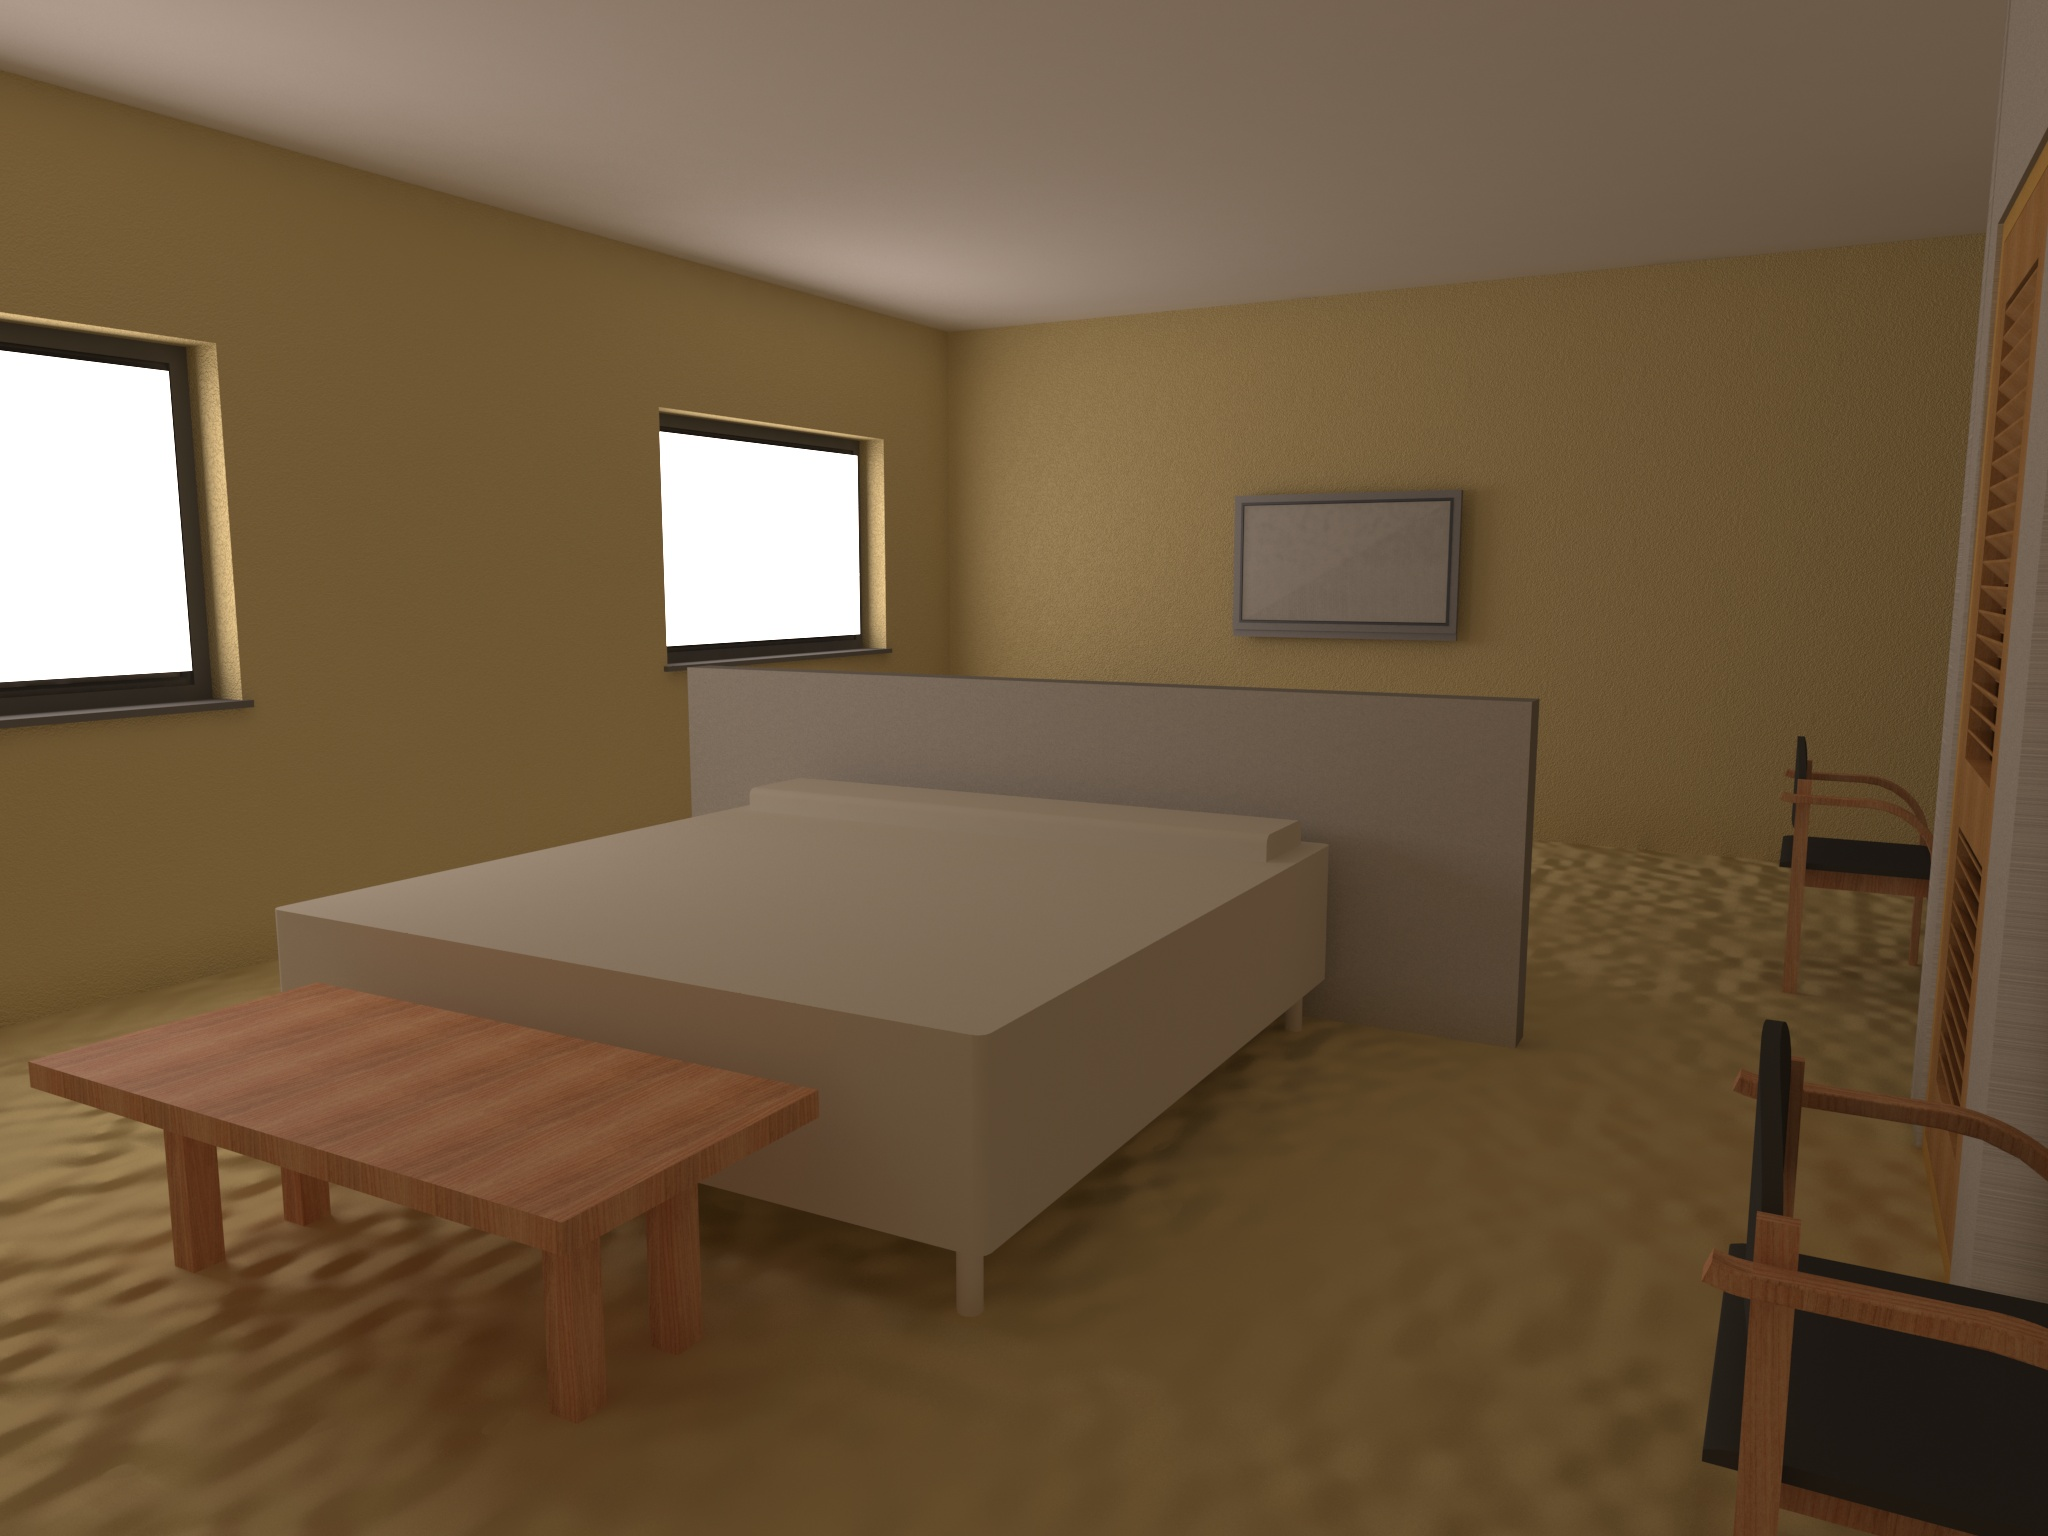
\includegraphics[width=10cm]{img/HotelRoomCamera1.jpg}
	\caption{Camera 5 Render}
	\label{fig:Cam5]}
\end{figure}


\\
\textbf{How to Structure your Submission}
\\
All submission are to take the form of a single zip file.  The zip file must maintain the folder structure as generated by 3DS Max or Unity.   The images below, figure \ref{fig:3dsstructure} and figure \ref{fig:unity} give an indication of the folder structure that you should zip and submit.\\ \\

\begin{figure}[h]
	\centering
	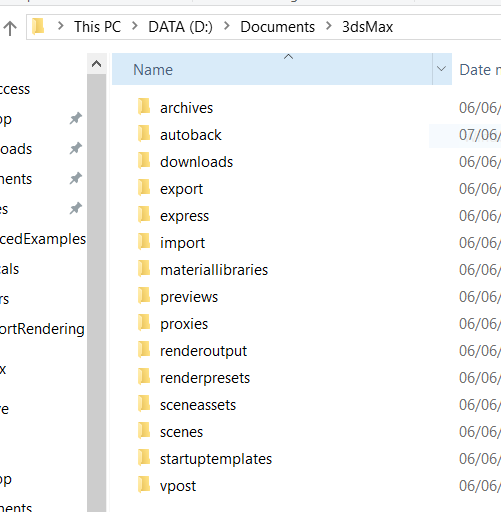
\includegraphics[width=0.5\linewidth]{img/3dsStructure.jpg}
	\caption{3D Studio Max Project Folder Structure}
	\label{fig:3dsstructure}
\end{figure}
\begin{figure}[h]
	\centering
	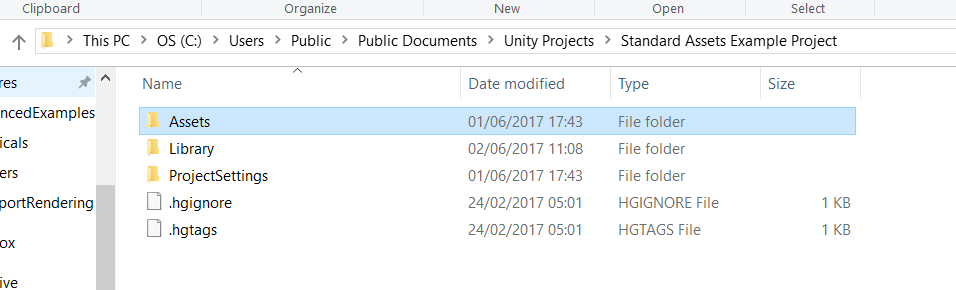
\includegraphics[width=0.9\linewidth]{img/Unity.jpg}
	\caption{Unity Game Engine File Structure}
	\label{fig:unity}
\end{figure}

All assets used during the course of the assignment are to be submitted.  All assets used and created should be placed within the appropriate folder.  To clarify, all 3ds Scene files should be placed within the 'scenes' folder; and all renders should be placed within the 'renderoutput' folder.
\\
\\
Please note that it is not appropriate to submit a single \textit{.max} file, single \textit{.jpg} file, or a single \textit{.unity} file.  

\vspace{1cm}
\textbf{Late Submission}\\
Failure to submit your assignment on or before the date and time indicated on Moodle will result in a penalty of 5\% per day or part thereof.
\\
\\
Late submission penalties will not apply in cases where a valid medical certificate is provided.  In such instances an extension of time will be granted for the duration of illness stated on the medical certificate that falls after the submission date.  A copy of the medical certificate must be included with the late submission.
\\
\\
Late submission penalties may also be avoided in exceptional circumstances.  These will be dealt with on a case by case basis.  Please note that loss of pen-drives, inability to use or access the software etc. will not be considered 'exceptional circumstances'.

\end{document}